%!TEX root = ../main.tex

\chapter{The ns-3 network simulator}
\label{chp:ns3}

\paragraph{}
The study behind this work required a thorough evaluation of a multitude of different non-terrestrial communication scenarios, that in turn required an extensive simulation campaign. Furthermore, the low-level nature of the issues that were expected to be found led to the need for a simulator that allowed access to the protocols' core implementation to be able to modify their behavior if needed. A simple API-level access to some protocols' attributes would have been not sufficient to implement all the suggested modifications.

\section{Description}
\label{sec:ns3_desc}

\begin{figure}[ht]
    \centering
    
\includegraphics[width=0.5\textwidth]{res/ns-3-notext.png}
    \caption{ns-3 logo \href{https://www.nsnam.org/}{nsnam.org}}
    \label{fig:ns3-logo}
\end{figure}

Being a modular, extensible, community-supported, full-stack network software simulation tool based on a discrete event approach, the ns-3 simulator was the software of choice to conduct the testing campaigns. It is an open source project licensed under the GNU GPLv2 license, meaning that the condition of being able to have full access to the source code to implement potential modifications is satisfied \cite{ns3-website}.

Other simulation pieces of software are available, such as OMNET++ (\href{https://omnetpp.org/}{omnetpp.org}), SWANS (\href{http://jist.ece.cornell.edu/}{jist.ece.cornell.edu}), NetSim (\href{https://www.tetcos.com/}{tetcos.com}), QualNet, and finally ns-3 predecessor, ns-2. Their main characteristics are summarized in Table \ref{tab:simulators}, from \cite{review-ns3}, which posed the accent on the suitability of ns-3 for research purposes, highlighting its success amongst the scientific community.

\subsubsection{Discrete events simulators}
In discrete-events simulators, each operation to be performed is associated to an event, and in turn, each event is associated with a set of instructions and its execution time. 

The simulation proceeds by processing and executing events, stepping from one to the next, as the simulation time passes. At the eyes of the simulation, each event is executed in zero time, since the time is stopped while executing a single event, and its course resumes only when transitioning between events scheduled at different times.

If no events are scheduled to execute for a certain period of time, the simulation immediately transitions to the next scheduled one. This kind of behavior is what discerns discrete events simulators from their counterparts,  real-time simulators.

As the simulation unfolds, it consumes events, but each executed event may generate new ones. As an example, the event of a packet being transmitted in a network may generate the corresponding reception event after a set propagation delay \cite{review-ns3}.

\begin{table}[]
    \small
    \begin{tabular}{|c|lllll}
        \hline
            {\ul \textbf{Tool}} &
            \multicolumn{1}{c|}{{\ul \textbf{ns-3}}} &
            \multicolumn{1}{c|}{{\ul \textbf{OMNET++}}} &
            \multicolumn{1}{c|}{{\ul \textbf{SWANS}}} &
            \multicolumn{1}{c|}{{\ul \textbf{NetSim}}} &
            \multicolumn{1}{c|}{{\ul \textbf{QualNet}}}
            \\ \hline

            {\ul Interface} &
            \begin{tabular}[c]{@{}l@{}}C++,\\ Python\end{tabular} &
            \begin{tabular}[c]{@{}l@{}}C++,\\ NED\end{tabular} &
            Java &
            \begin{tabular}[c]{@{}l@{}}C,\\ Java,\\ .NET\end{tabular} &
            Parsec
            \\ \hline

            {\ul License} &
            Free &
            Academic &
            Free &
            Paid &
            Paid
            \\ \hline
            
            {\ul Parallelism} &
            No &
            No &
            Yes &
            No &
            Yes
            \\ \hline

            {\ul OS} &
            \begin{tabular}[c]{@{}l@{}}Linux,\\ FreeBSD,\\ MacOS\\ Windows\end{tabular} &
            \begin{tabular}[c]{@{}l@{}}Linux,\\ MacOS,\\ Windows\end{tabular} &
            \begin{tabular}[c]{@{}l@{}}Linux,\\ MacOS,\\ Windows\end{tabular} &
            Windows &
            \begin{tabular}[c]{@{}l@{}}Linux,\\ MacOS,\\ Windows,\\ Unix\end{tabular}
            \\ \hline

            {\ul Mobility support} &
            Yes &
            No &
            Yes &
            Yes &
            Yes
            \\ \hline

            {\ul GUI} &
            Limited &
            Yes &
            Yes &
            Yes &
            Yes
            \\ \hline
    \end{tabular}
    \caption{Network simulation software comparison \label{tab:simulators}}
\end{table}

\subsubsection{The community}
Being specifically targeted for the academic world and research purposes, as well as being open-source, ns-3 sees a thriving community of developers and researchers, with an active forum\footnote{Link to google group about ns-3 \href{https://groups.google.com/g/ns-3-users}{groups.google.com/g/ns-3-users}}, a well maintained documentation and a lot of independent lectures, tutorials and articles. 


\section{NTN module}

\subsection{Channel model}
In \cite{3gpp-tr-38.821}, \ac{3GPP} defines different standard reference scenarios to be considered when evaluating non-terrestrial networks. Such scenarios and their conditions are listed in Table \ref{tab:scenarios}. Moreover, a key factor for non-terrestrial communication is whether the ground terminal is able to view the satellite, called \ac{LOS} condition. Each scenario can therefore be further divided basing on the two different sights possibilities.

\subsubsection{Free space path loss}
The free space path loss is the major attenuation component in non-terrestrial links due to the long involved distances, and can be calculated as the ratio between the received power and the transmitted power with the well-known Friis formula 

\begin{equation}
    \frac{P_r}{P_t} = D_tD_r\left(\frac{\lambda}{4\pi d}\right)^2
    \label{eqn:fspl}
\end{equation}

Where $D_t$ and $D_r$ denote the directivities of the transmitting and receiving antennas, $\lambda$ is the wavelength and $d$ the distance.


\subsubsection{Atmospheric attenuation}
\paragraph{}
In addition to the free-space path loss that characterizes the majority of wireless communication systems, atmospheric absorption also plays an important role in attenuating certain frequency bands of the signal. Figure \ref{fig:atmospheric-abs} from \cite{e-band-ammar} details the behavior of atmospheric absorption in the mm-Wave frequency range. The peaks at 60 and 120GHz are due to the resonance with molecular oxygen, while the peak at 180GHz and the small hump at 25GHz are due to the absorption from water vapor \cite{e-band-ammar}.

The nature of this phenomenon makes it susceptible to variations as the humidity rate varies, and different altitudes also lead to different absorption values.

\subsubsection{Shadowing}
Shadowing is the effect of the signal being reflected and scattered by surrounding objects, therefore arriving at the receiving antenna from many different paths. This causes multiple copies of the signal to be received, each copy having its own attenuation and phase, since the travelled path, and therefore distance, can be different. This behavior can rapidly fluctuate, generating both constructive or destructive interference.

\subsubsection{Other factors}
Other factors causing additional attenuation are the presence of rain, cloudy conditions, the presence of fog, and different meteorological parameters. These factors are described in \cite{atm-effects-signal-prop}.

Furthermore, the different scenarios that the \ac{UE} can experience also have a major impact on its communication capabilities. Such scenarios are divided by \ac{3GPP} in four main categories: Dense urban, Urban, Suburban and Rural. In each scenario, the probability of having direct \ac{LOS} with a satellite differs, since the density of obstacles such as buildings varies depending on the situation.



\begin{figure}[ht]
    \centering
    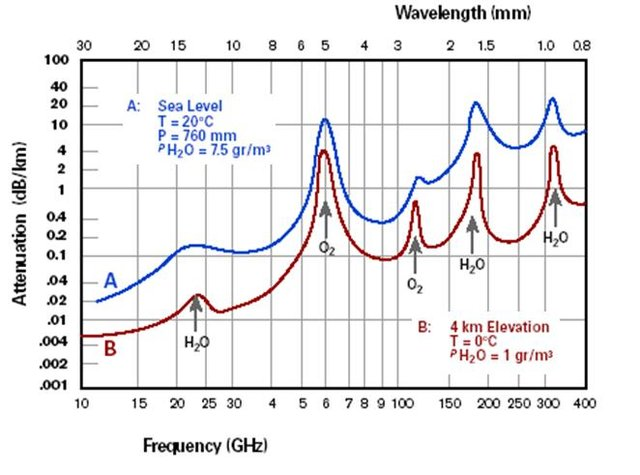
\includegraphics[width=0.8\textwidth]{res/atm-absorp.jpg}
    \caption{Atmospheric absorption in dB per kilometer, from \cite{e-band-ammar}}
    \label{fig:atmospheric-abs}
\end{figure}



\begin{table}[]
    \begin{tabular}{cllll}
    \hline
    {\ul \textbf{Case}} & \multicolumn{1}{c}{{\ul \textbf{Orbit}}} & \multicolumn{1}{c}{{\ul \textbf{Terminal}}} & \multicolumn{1}{c}{{\ul \textbf{Band}}} & \multicolumn{1}{c}{{\ul \textbf{Polarization Reuse}}} \\ \hline
    1  & GEO      & VSAT     & Ka & Disabled \\ \hline
    2  & GEO      & VSAT     & Ka & Enabled  \\ \hline
    3  & GEO      & VSAT     & Ka & Enabled  \\ \hline
    4  & GEO      & Handheld & S  & Disabled \\ \hline
    5  & GEO      & Handheld & S  & Enabled  \\ \hline
    6  & LEO-600  & VSAT     & Ka & Disabled \\ \hline
    7  & LEO-600  & VSAT     & Ka & Enabled  \\ \hline
    8  & LEO-600  & VSAT     & Ka & Enabled  \\ \hline
    9  & LEO-600  & Handheld & S  & Disabled \\ \hline
    10 & LEO-600  & Handheld & S  & Enabled  \\ \hline
    11 & LEO-1200 & VSAT     & Ka & Disabled \\ \hline
    12 & LEO-1200 & VSAT     & Ka & Enabled  \\ \hline
    13 & LEO-1200 & VSAT     & Ka & Enabled  \\ \hline
    14 & LEO-1200 & Handheld & S  & Disabled \\ \hline
    15 & LEO-1200 & Handheld & S  & Enabled  \\ \hline
    \end{tabular}
    \caption{3GPP scenarios for NTN \label{tab:scenarios}}
    \end{table}

\subsection{NS-3 channel model implementation}

\paragraph{}
Work on a ns-3 module to allow simulations in non-terrestrial scenarios to be properly conducted is already in progress, and considerable effort has been put in the realization of a non-terrestrial channel model\footnote{The code is available at the following repository: \href{https://gitlab.com/mattiasandri/ns-3-ntn/-/tree/ntn-dev?ref_type=heads}{gitlab.com/mattiasandri}}.

The implementation of such channel model required the modification and the creation of some ns-3 classes. This work is extensively described in \cite{Sandri_2023}, while a brief overview is hereby reported.

\subsubsection{Modified classes}
\begin{itemize}
    \item \texttt{ThreeGppChannelModel}: different parameters were introduced in order for this class to be able to correctly characterize the non-terrestrial use case. The large number of \ac{NTN}-related parameters made necessary the use of data structures such as maps to store them, and the mobility model of both the satellite and the \ac{UE} have been integrated in the computation of the small scale parameters returned by the class.
    \item \texttt{GeographicPositions}: class tasked with the various conversions between different coordinates systems such as longitude, latitude and altitude, the Geocentric Cartesian system (also called Earth Centric Earth Fixed or ECEF), and the local tangent plane coordinate system expressing the position in North, East and Up coordinates \cite{wiki_coords}. All those three systems are depicted in Fig. \ref{fig:coord-syst}.
\end{itemize}
\subsubsection{New classes}
\begin{itemize}
    \item \texttt{ThreeGppNTNScenarioChannelConditionModel}: the main task of this class is to store the channel state and condition. Four new classes were written to store the four possible scenarios described by \ac{3GPP}:
    \begin{itemize}
        \item Dense urban,
        \item urban,
        \item suburban,
        \item rural
    \end{itemize}
    \item \texttt{ThreeGppNTNScenarioPropagationLossModel}: once again, four different scenarios are implemented in as many classes. Such classes are tasked with the computation of the total path loss, which includes contributions from the standard free space path loss, atmospheric absorption, scintillation, fading and clutter loss.
    \item \texttt{GeocentricConstantPositionMobilityModel}: mainly helps position \ac{UE}s on the Earth surface in an easier way by allowing it to be input in a more natural coordinate set. Conversions amongst different systems are done using the \texttt{GeographicPositions} class described above.
    \item \texttt{CircularApertureAntennaModel}: a more precise implementation of the default ns-3's parabolic antenna model, this time making use of a newer and more efficient C++ function for the computation of Bessel functions required when considering the radiation pattern of aperture antennas \cite{rad-patterns}.
\end{itemize}




\begin{figure}[ht]
    \centering
    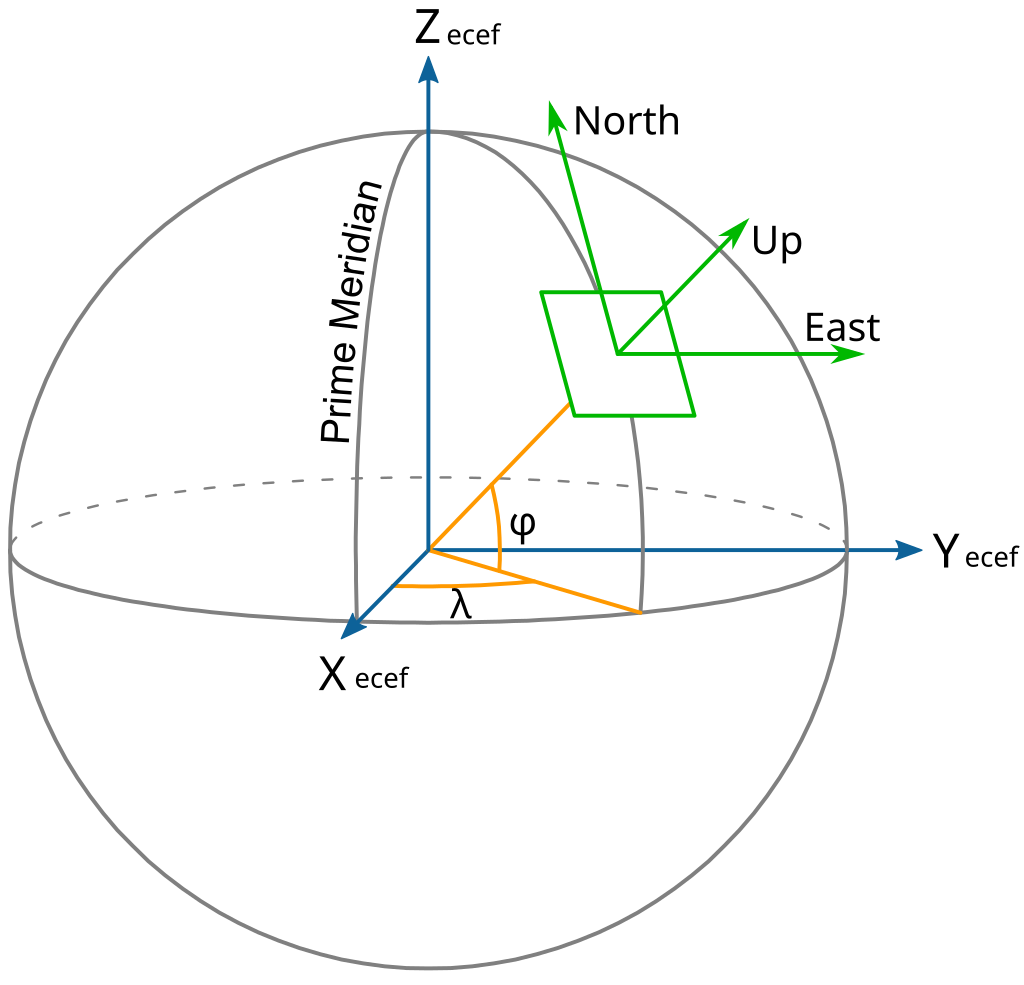
\includegraphics[width=0.8\textwidth]{res/coord_systems.png}
    \caption{Showcase of different coordinates systems \cite{wiki_coords}}
    \label{fig:coord-syst}
\end{figure}

\subsubsection{Use in this work}
\paragraph{}
All the aforementioned implementation is based on the \ac{3GPP} specifications as detailed in the standard \cite{3gpp-tr-38.811}, and the resulting channel model enables full-stack end-to-end simulations considering different \ac{NTN} scenarios \cite{Sandri_2023}.

This work can therefore benefit from an already existing standard implementation of the channel model, a crucial point for its aim of providing a simulation of how the complete \ac{NR} protocol stack would behave in such a challenging scenario. 

\section{Implemented scenario}

This section aims at describing the reference scenario that was implemented in the ns-3 simulator in order to test the \ac{NR} protocol suite in a non-terrestrial communication setting.

\subsection{Network topology}
To conduct the various simulation campaigns, ensuring the reproducibility and the comparability of the obtained results, a reference network topology has been made, and the parameters specified by \ac{3GPP} have been used.

The simple network setup is depicted in Fig. \ref{fig:sim-scenario} and it consists of the following elements:
\begin{itemize}
    \item \textbf{Packet source}: application installed on the user equipment that generates packets with a specified periodicity. Both the generation rate and the packets' size can be varied by acting on their respective parameters. All the other variables that can be controlled are listed in the code snippet \ref{code:ue_parameters}
    \item \textbf{UE antenna}: the transmission of data is performed by mean of a \ac{vSAT} antenna placed at the \ac{UE} side. The main parameters of such antenna are found in the code snippet \ref{code:tx_parameters}.
    \item \textbf{Non-terrestrial link}: link connecting the \ac{UE} placed on the ground with the \ac{gNB}. This wireless link is characterized its propagation delay, bandwidth and frequency. However, since the aim of this work is to study the effects of propagation delay on the protocol suite, the bandwidth and frequency remained constant across all the simulations to better isolate the variables that could potentially cause problems. The list of parameters can be found in the code snippet \ref{code:link_parameters}.
    \item \textbf{g-NodeB}: the adopted approach is to incorporate the g-NodeB into the satellite payload, therefore adopting the configuration described in section \ref{sec:onboard-gnb}. This decision was made since the high one-way propagation delay is enough to cause some of the involved protocols to start malfunctioning. Adopting the bent-pipe configuration described in \ref{sec:bent-pipe-payload} would have resulted in effectively doubling the delay between \ac{UE} and \ac{gNB}. The satellite aperture antenna parameters follow the ones specified in the scenario named "10 DL" described in \cite{3gpp-tr-38.821}, and are listed in the code snippet \ref{code:sat_parameters}.
    \item \textbf{High performance link}: link connecting the g-NodeB to the packet sink. This is part of 5G core network, and it shall not be causing any additional problems, since that would be out of the scope of this work. This link was therefore meant to be as close as possible to an ideal one, with a capacity of 100Gb/s, a \ac{MTU} of 1500B and a delay of a single microsecond.
    \item \textbf{Remote host}: packet sink representing the destination node of all the packets generated at the \ac{UE}.
\end{itemize}



\begin{lstlisting}[language=C++, caption=Application and UE configuration parameters, label=code:ue_parameters]
    bool enableNagle = false;  // whether to enable Nagle's algorithm
    bool enableHarq = false;   // whether to enable HARQ protocol
    uint32_t numHarq = 100;    // max number of concurrent HARQ processes
    uint32_t harqTimeout = 10; // timeout for HARQ processes
    bool rrcIdeal = false;     // use ideal version of RRC protocol
    double tcpMinRto = 200;             // minimum TCP RTO
    uint32_t tcpBufSize = 131072 * 100; // TCP buffer size
    double ipv4FrExpTimeout = 200;      // IPv4 fragment expiration timeout
    double perr = 0.1;                  // target error probability when transmitting PHY-level packets

    // Application parameters
    std::string transportPrtcl = "UDP"; // Whether to use UDP or TCP
    uint32_t numPackets = 2000;         // max number of packets to be sent
    double appStartTimeSec = 0.5;       // application start time
    double appStopTimeSec = 5.5;        // application stop time
    double simStopTimeSec = 6;          // simulation stop time
    uint32_t packetSizeBytes = 200;     // application packets' size
\end{lstlisting}

\begin{lstlisting}[language=C++, caption=UE antenna parameters, label=code:tx_parameters]
    // UE Parameters
    double vsatAntennaGain = 39.7;       // dB
    double vsatAntennaDiameter = 0.6;    // meters
    double vsatAntennaNoiseFigure = 1.2; // dB 
\end{lstlisting}

\begin{lstlisting}[language=C++, caption=Satellite antenna parameters, label=code:sat_parameters]
    // Satellite parameters
    double satEIRPDensity = 40;    // dBW/MHz
    double satAntennaGain = 58.5;  // dB
    double satAntennaDiameter = 5; // meters
    double distance = -1;          // height of the satellite in km
\end{lstlisting}

\begin{lstlisting}[language=C++, caption=Non-terrestrial link parameters, label=code:link_parameters]
    uint64_t propDelay = 6;     // propagation delay in ms
    double frequency = 20e9;    // link carrier frequency
    double bandwidth = 400e6;   // link bandwidth
\end{lstlisting}

\begin{figure}[ht]
    \centering
    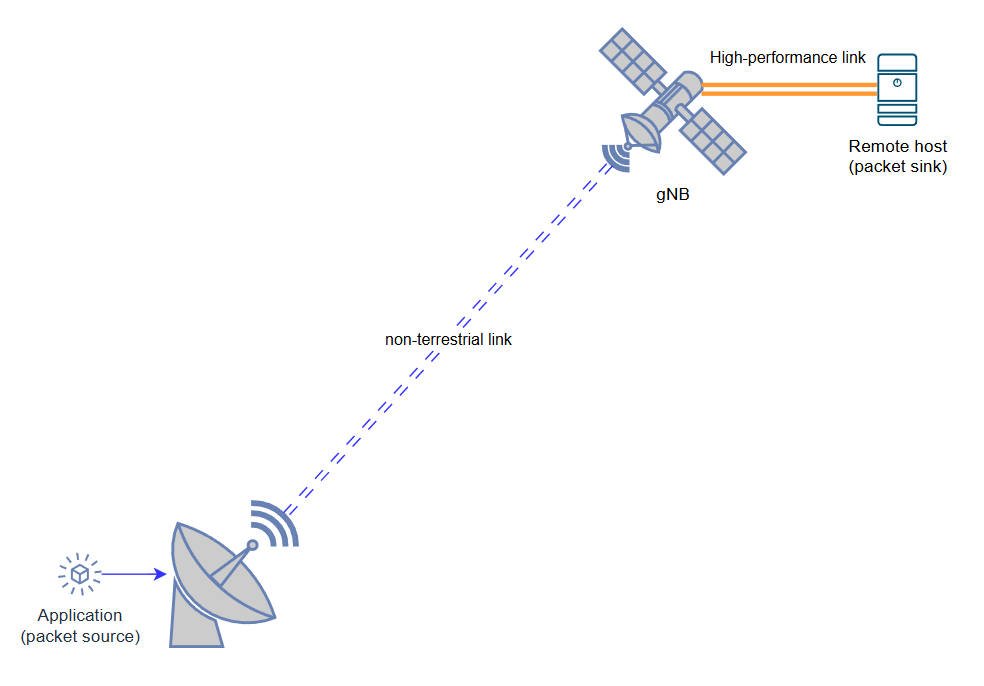
\includegraphics[width=0.8\textwidth]{res/sim-scenario.png}
    \caption{Network simulation scenario}
    \label{fig:sim-scenario}
\end{figure}